\section{Dataset overview}
\label{sec:dataset}

We 
%collect, align, and release 
derive 
a suitable dataset for melody transcription using crowdsourced annotations from \hooktheory{}.\footnote{\hooktheory{} annotations are published under a \href{https://creativecommons.org/licenses/by-nc-sa/3.0/}{CC BY-NC-SA 3.0} license, which our dataset inherits.}
\hooktheory{} is a platform where users can easily create and share musical analyses of particular recordings hosted on YouTube, with Wikipedia-style editing. 
In lieu of a precise technical definition, these melody annotations constitute a working definition of what musicians perceive as melody. 
The dataset contains annotations for $22$k segments of $13$k unique recordings totaling $50$ hours of labeled audio. 
The audio content covers a wide range of genres---there is a skew towards pop and rock but many other genres are represented including EDM, jazz, and even classical. 
We create an artist-stratified $8$:$1$:$1$ split of the dataset for training, validation, and testing. 
The dataset also includes chord annotations which may facilitate chord recognition research.

% Note that the melody annotations originate from a software tool which uses a ``functional'' annotation format, i.e.,~one which uses scale degrees and roman numerals relative to a key signature instead of absolute notes and chord names. 
% The vast majority of transcription work uses absolute labels, hence, we convert these functional labels to absolute ones. 
% However, because the annotation tool uses a relative octave format, there is no way to reliably map the melody annotations to the ground truth absolute octave. 
% The disregard of absolute octave information on this popular annotation platform implies that a crowd definition of melody does not include this information, reinforcing our earlier argument that it should be ignored for evaluation.

%\john{Should this paragraph come at the end of the section?}
While data from \hooktheory{} has been used previously for MIR tasks like 
harmonization~\cite{chen2021surprisenet,yeh2021automatic}, 
chord recognition~\cite{jiang2019mirex}, and 
representation learning~\cite{jiang2020transformer}, 
making use of this platform for MIR is currently cumbersome. 
One obstacle is that the raw annotations are created via a ``functional'' interface, i.e.,~one which uses scale degrees and roman numerals relative to a key signature instead of absolute notes and chord names. 
In contrast, most MIR research favors absolute labels.
Hence, we convert these annotations from their proprietary functional format to a simple (JSON-based) absolute format. 
One caveat is that the \hooktheory{} annotation interface uses a relative octave system, 
so there is no way to reliably map the annotations to their ground truth octave.
Thus, melodies in our dataset also contain only relative octave information.

\begin{figure}
    \centering
    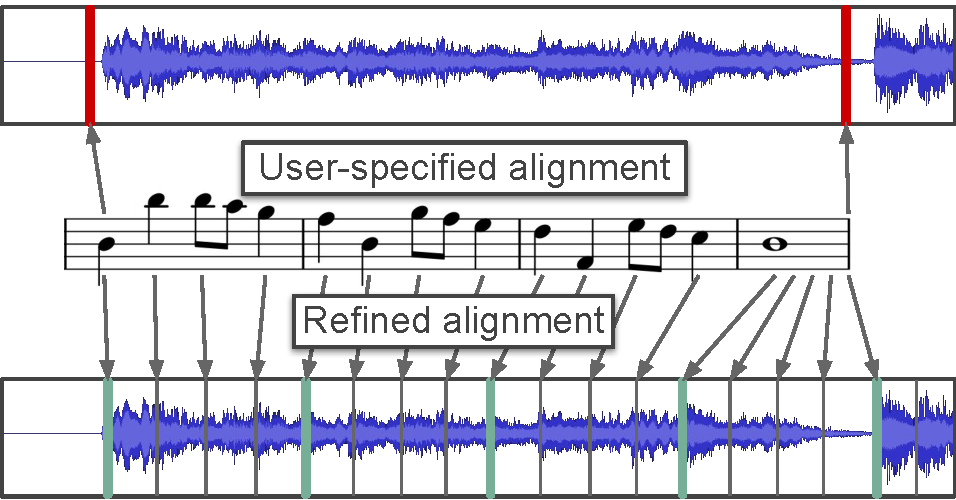
\includegraphics[width=8.1cm]{figs/alignment.pdf}
    \caption{We refine the crude user-specified alignments from \hooktheory{} by using beat and downbeat tracking. The first segment beat is mapped to the detected downbeat nearest to the user-specified starting timestamp, and remaining beats are mapped to subsequent detected beats.}
 \label{fig:alignment}
\end{figure}

An additional obstacle specific to transcription is that the alignments between the audio and the annotations are crude---users provide only an approximate starting and ending timestamp of their annotated segment within the audio. 
Because transcription methodology generally depends on precise alignments, we make an effort to refine the user-specified ones. 
To this end, we make use of the beat and downbeat detection algorithm from \madmom{}~\cite{bock2016joint,bock2016madmom}. 
Specifically, our approach aligns the first beat of the segment to the detected downbeat which is nearest to the user-specified starting timestamp. 
Then, we align the remaining beats to the subsequent detected beats (see~\Cref{fig:alignment} for an example). 
This provides a beat-level alignment for the entire segment, which we linear interpolate to fractional subdivisions of the beat. 
Formally, we construct an alignment function $\texttt{Align} : [0,B) \to [0,T)$ that assigns each of $B$ beats in the metrical structure to a time $t \in [0,T)$ in the audio.
In an informal listening test, this produces an improved alignment in around $95\%$ of cases, where the primary failure mode in the remaining $5\%$ occurs when \madmom{} detects the wrong beat as the downbeat. 
We use these refined alignments for training and evaluation and release them alongside the dataset.
%, accepting the occasional glitched alignments as noise in the dataset.